%%%%%%%%%%%%%%%%%%%%%%%%%%%%%%%%%%%%%%%%%%%%%%%%%%%
%
%  New template code for TAMU Theses and Dissertations starting Fall 2012.  
%  For more info about this template or the 
%  TAMU LaTeX User's Group, see http://www.howdy.me/.
%
%  Author: Wendy Lynn Turner 
%	 Version 1.0 
%  Last updated 8/5/2012
%
%%%%%%%%%%%%%%%%%%%%%%%%%%%%%%%%%%%%%%%%%%%%%%%%%%%

%%%%%%%%%%%%%%%%%%%%%%%%%%%%%%%%%%%%%%%%%%%%%%%%%%%%%%%%%%%%%%%%%%%%%%%
%%%                           SECTION I
%%%%%%%%%%%%%%%%%%%%%%%%%%%%%%%%%%%%%%%%%%%%%%%%%%%%%%%%%%%%%%%%%%%%%%

\renewcommand*{\thefootnote}{\fnsymbol{footnote}}
\chapter[\uppercase{Targeted Observations with the VIRUS Prototype Instrument}]{\uppercase{Targeted Observations with the VIRUS Prototype Instrument}\symbolfootnote[1]{Reprinted with permission from ``Introduction: The Importance of Research'' by AUTHOR et al., 2015. The Astrophysical Journal, Volume XYZ, Issue X, article id. XY, XY pp., Copyright 20XX by the American Astronomical Society.} }
\renewcommand*{\thefootnote}{\arabic{footnote}}
\setcounter{footnote}{0}

\section{Introduction} 
Clusters of galaxies form the largest bound objects in the universe, and as such their study is a cornerstone in modern day astronomy. Thought to form out of the primordial density fluctuations in the very early universe \citeeg{Press1974}, the number and distribution of galaxy clusters across the sky is the finger print of the cosmology imprinted on the universe at its birth.

Many large area-sky surveys both currently underway and upcoming are prioritizing the identification of clusters for both detailed studies of cosmology and for fundamental physical studies of the individual clusters. At present, the greatest number of clusters are being discovered using large millimeter wave surveys with the South Pole Telescope (SPT; \citealt{Carlstrom2011}) or the Atacama Cosmology Telescope (ACT; \citealt{Swetz2011}). These observations rely on the Sunyaev-Zel'dovich effect (SZE; \citealt{Sunyaev1972}) which uses the up-scattering of cosmic microwave background (CMB) photons to both identify the cluster and to estimate its mass. However, deep, wide field optical surveys, such as the Dark Energy Survey (DES; \citealt{DES2005}) and planned Large Synoptic Survey Telescope (LSST; \citealt{LSST2012}) will discover many more clusters at increasing lower mass in the near future. Such clusters will rely on follow up to better constrain their dynamical mass. But, as the number of clusters grows to many tens of thousands, individual followup becomes unfeasible. Therefore, we rely on well calibrated observable-mass relationships to estimate the masses of the observed clusters.

Unfortunately, mass is not directly observable, so we must estimate it through another observable. Observed X-ray temperatures and luminosities correlate tightly with a cluster's dynamical mass \citeeg{Mantz2010, Rykoff2014}, especially for dynamically relaxed clusters \citeeg{Mantz2015}. Observations of the SZE can provide accurate estimations of mass \citeeg{Vanderlinde2010, Sehgal2011}, but can be effected by the physics of the intracluster medium \citeeg{Pipino2010} and the ability to detect low mass galaxy clusters is currently limited by technology \citeeg{Carlstrom2002a}. The richness \citeeg{Abell1958,Rykoff2012}, the weighted number of cluster member galaxies within a scale aperture, is a promising method which has been shown to correlate strongly with cluster mass \citeeg{Rozo2010}. 

Of the methods listed, the richness is most promising for future large area-sky surveys as it relies on photometry only. It is already being used in many optical studies \citeeg{Ruel2014, Sifon2015}, but the absolute mass scale and more importantly the  intrinsic scatter in the relation are currently under active investigation \citeeg{Rozo2015, Saro2015, Baxter2016, Farahi2016, Simet2016}. These systematics remain the major source of uncertainty in deriving cosmological constraints from cluster abundances and testing structure growth in a $\Lambda$CDM universe. To realize fully the promise of the large samples from DES and LSST, we must measure both the absolute mass scale and scatter in the optical-richness mass estimator using independent methods.

In this work, we present a pilot study of ten massive galaxy clusters using integral field spectroscopy with the Mitchell Spectrograph as a pilot program for the Hobby Eberly Dark Energy Experiment (HETDEX; \citealt{Hill2008}). HETDEX is a forthcoming blind spectroscopic survey that could potentially be used to accurately calibrate the optical richness-mass relation for a significant number of galaxy clusters at both extremes of the mass scale. At present, because HETDEX is designed to measure the dark energy equation of state at $z\sim2$, and the applicability to galaxy cluster science has not yet been investigated. We began this investigation with \defcitealias{Boada2016}{Paper I}\cite{Boada2016} (hereafter \citetalias{Boada2016}). The second installment of this two part work, the goal of this study is to obtain spectroscopic redshifts of the individual cluster galaxies, determine the velocity dispersion and to infer each cluster's dynamical mass. This allows us to compare the inferred mass with other mass estimators (\eg, the clusters in this sample have deep \textit{Chandra} or \textit{XMM-Newton} X-ray data, and richness measurements) with the aim of better characterizing the scatter in the richness-mass relation, $\sigma_{M|\lambda}$. The ability of HETDEX to further constrain optically derived masses is of paramount importance to upcoming large photometric surveys. This study provides insight into how well a HETDEX type survey will constrain mass estimations and cosmological parameters in the future.

The layout of this work is the following. In Section~\ref{2sec:design} we discuss the target selection and the setup of the Mitchell Spectrograph used to conduct the observations. Section~\ref{2sec:data reduction} describes the methods and tools used to reduce the observations. We present our redshift catalog, cluster members and cluster dynamical properties in Section~\ref{2sec:analysis}. We discuss a machine learning based alternative to a traditional power law estimate of cluster mass in Section~\ref{2sec:ML methods} In Section~\ref{2sec:results}, we compare and discuss the different mass estimations and remark on the applicability of these methods for the study of the optical richness-cluster mass relationship.  Finally, we summarize this work in Section~\ref{2sec:summary}.

Throughout this paper, we adopt the following cosmological model: $\Omega_\Lambda = 0.714$, $\Omega_M = 0.286$, $\sigma_8 = 0.82$ and $H_0= 70$ \kms \mpc, assume a Chabrier initial mass function (IMF; \citealt{Chabrier2003}), and use AB magnitudes \citep{Oke1974}.

\section{Design}\label{2sec:design} 
\subsection{Target Selection}\label{2sec:selection} 
We select clusters at $z=0.2-0.3$ using two different methods and for two different purposes. Eight of the ten clusters are optically selected from \cite{Rykoff2012} using the \textit{Sloan Digital Sky Survey} (SDSS; \citealt{Blanton2001a}) Data Release 8. These clusters have high ($M_{DM} > 8\times10^{14}\msol$) optically traced mass (richness; discussed further below), and are a combination of relaxed and unrelaxed systems. The last two clusters are selected from the \textit{XMM Cluster Survey} (XCS; \citealt{Mehrtens2012}) and correspond to individually measured X-ray temperatures of $T_X < 2.5$ keV. Such X-ray temperatures have inferred masses of $10^{14}\msol > M_{DM} > 5\times10^{13}\Msol$.

\begin{landscape}
	\begin{table}
		\caption{Basic properties of the ten galaxy clusters targeted with the MS: Column 1: Our internal cluster name; Column 2: An alternative cluster name; Column 3: The right ascension of the cluster; Column 4: The declination of the cluster; Column 5: the nominal (often photometric) cluster redshift; Column 6: The date of our observations.} 
		\begin{tabular}
			{lccccc} \hline Cluster & Alt. Name & RA (J2000) & DEC (J2000) & $z$ & Obs. Date\\
			(1) & (2) & (3) & (4) & (5) & (6) \\
			\hline \hline
			c16p23+0p06 & SOGRAS J0104+0003 & 01:04:55.369 & +00:03:36.28 & 0.277 & August, 2012 \\
			c203p83+41p0 & Abell 1763 & 13:35:20.092 & +41:00:04.12 & 0.223 & May, 2012 \\
			c210p2+02p8 & Abell 1835 & 14:01:01.965 & +02:52:42.63 & 0.252 & May, 2012 \\
			c234p2+24p4 & MaxBCG J234.23439+24.40877 & 15:36:56.253 & +24:24:31.60 & 0.226 & May, 2012 \\ 
			c250p08+46p7 & Abell 2219 & 16:40:19.812 & +46:42:41.51 & 0.225 & May, 2012 \\
			c260p61+32p13 & Abell 2261 & 17:22:27.182 & +32:07:57.24 & 0.224 & May, 2012 \\
			c319p70+0p56 & MaxBCG J319.70446+00.56035 & 21:18:49.069 & +00:33:37.33 & 0.270 & August, 2012 \\
			c328p33+0p19 & Abell 2392 & 21:54:22.936 & +00:37:23.48 & 0.223 & August, 2012\\
			XMMXCSJ124425.9+164758.0 & WHL J124425.4+164756 & 12:44:25.203 & +16:47:48.00 & 0.235 & May, 2013 \\
			XMMXCSJ125650.2+254803.2 & \nd & 12:56:49.999 & +25:48:02.99 & 0.280 & May, 2013 \\
			\hline 
		\end{tabular}
		\label{2tbl:targets} 
	\end{table}
\end{landscape}

The optically selected clusters have many more members (see Table~\ref{2tbl: derived parameters}) than the X-ray selected clusters which allows us to investigate the accuracy of our mass recovery methods at both cluster and group scales. See Table~\ref{2tbl:targets} for individual cluster sky positions and associated parameters. 

\subsection{The Mitchell Spectrograph} 
The Mitchell Spectrograph (MS; formerly known as VIRUS-P; \citealt{Hill2008a}) is an integral field unit (IFU) in a square array of 246 $4\farcs24$ diameter optical fibers. This provides a $1\farcm7~\times~1\farcm7$ field-of-view (FOV) with a 1/3 filling factor. A Fairchild Instruments, 2k$\times$2k charge couple device (CCD) images the spectra from each of the 246 fibers. The spectra have approximately a gaussian profile with a 5 pixel full width at half maximum (FWHM), and each are separated by 8 pixels to minimize the amount of cross-talk between the fibers. 

There are two spectral configurations available on MS, a blue setup, 3600-5800 \AA\ and a red setup, 4600-6800 \AA. In addition, there are four volume phase holographic gratings available to disperse the light. For the purpose of this work, the lowest resolution, $\sim5$\AA, grating is used. Using $1\times1$ binning, this translates into a spectral dispersion of $\sim1.11$ \AA\ pixel$^{-1}$. 

\subsection{Observations} 
\begin{figure}[t]
	\begin{center}
		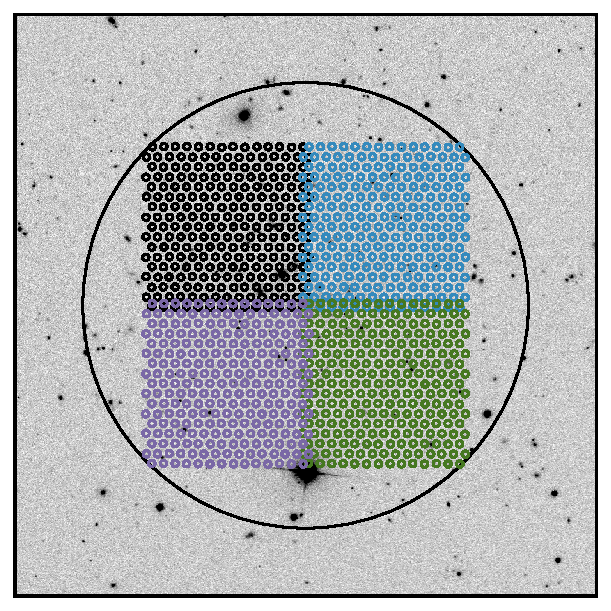
\includegraphics[width=0.6\textwidth]{./figures2/pointing.pdf} 
	\end{center}
	\caption{Example cluster observations}
	SDSS r-band image of an optically selected galaxy cluster selected from the SDSS DR8 data. The field is centered on the BCG, which has a measured spectroscopic redshift from SDSS of $z = 0.277$. The large black circle shows the region $R<0.5$ Mpc ($r<2\farcm3$). Nearly all galaxies within this region are associated with the cluster. The four MS fields (and fiber positions for the first dither position) are overdrawn on the field, illustrating how we survey each cluster. \label{2fig:tiles} 
\end{figure}

We use MS to target the galaxy clusters using the 5 \AAA\ grating covering a wavelength range of $4400 - 6600\AAA$. With this instrumental setup and for galaxies $z = 0.2-0.3$, we will cover the Ca H\&K, \hbox{\ion{Fe}{i}} ($\lambda 4383$), H-$\delta$, H-$\gamma$ and H-$\beta$ absorption features. Additionally, we cover emission of the \hbox{[\ion{O}{ii}]} ($\lambda\lambda 3727,3729$) doublet, H-$\beta$, and \hbox{[\ion{O}{iii}]} ($\lambda\lambda 4960,5008$), which allows for the identification of actively star-forming galaxies.

The FOV of the MS corresponds to an approximately 0.4 Mpc square region at $z = 0.2-0.3$. To ensure adequate coverage of the cluster out to a radius of 0.5 Mpc, we use four MS pointings per cluster. Figure~\ref{2fig:tiles} shows an example of the pointing pattern done on each cluster. The northeast, northwest, southwest, and southeast fields with the fiber positions are shown in black, blue, green and purple respectively. The entire field is centered on the brightest cluster galaxy (BCG) and the individual tiles are shifted away. Furthermore, each of the four tiles are dithered at relative positions $(\Delta \alpha, \Delta \delta)=(0\farcs0,0\farcs0)$, $(-3\farcs6,-2\farcs0)$, and $(0\farcs0, -4\farcs0)$ from the origin to ensure full coverage of the FOV. Therefore, there are 736 individual spectra for each of the four fields or 2952 measurements for the cluster as a whole.

We have set exposure times to achieve spectra with signal-to-noise ratios (SNRs) $\sim3$ per spectral element in the continuum for objects with \sdssg\ $= 21.3$ mag (which corresponds to approximately 0.2L$^\star$ for cluster galaxies at $z = 0.2$). We base the expected SNR on the experience of \cite{Shetrone2010}, who achieves SNR $= 100$ per pixel in the continuum for point sources with B $=16.5$ mag at 4000 \AAA\ in 4800 seconds. Therefore, for our faintest objects with B $\approx$ g $= 21.3$ mag, we expect to achieve SNR $= 3$ per spectral element (averaged over 4.6 pixels) in 3600 seconds per pointing. We require 4 pointings to cover the full area for each cluster. Therefore, we require 1 hr/pointing $\times$ 4 pointings $= 4$ hrs on sky per cluster. Even though the field is dense with galaxies, there is sufficient ``blank'' area to allow for enough ``sky'' fibers for background subtraction. Therefore, no individual ``sky'' exposures are required.

\section{Data Reduction}\label{2sec:data reduction} 
All data are reduced using \textsc{p3d}\footnote{http://p3d.sourceforge.net/} \citep{Sandin2010} a general-use IFU reduction pipeline. The first step is to min/max-filtered average combine a minimum of 20 bias images from each night into a master-bias image, which is subtracted from each other image from the same night. Secondly, a trace mask is created from flat-fielding on the dusk or dawn sky. The fibers are fairly densely packed, so to determine the position of each spectrum in the dispersion direction each spectrum is extracted using a multi-profile deconvolution approach \citep{Sharp2010} to account for cross talk between fibers. Third, a dispersion mask for the wavelength calibration from images of Hg+Cd (for the May, 2012 observations) or Cd+Ne (for all other observations) arc lamps. The residuals between the derived wavelength solution and the known wavelengths of the emission lines is calculated from a fifth order polynomial and lie between $0.02 - 0.06$ \AAA. Finally, a fiber flat is created from the sky flats by a min/max-filtered average combine as in step one. 

All that remains is the extraction of the science images, however there are several steps in this process. First, the science frames are bias subtracted. Next each frame is cleaned of cosmic ray hits using the \textsc{PyCosmic} \citep{Husemann2012} integrated into \textsc{p3d} with the default parameters. Third the extracted spectra are wavelength calibrated using the previously created dispersion mask. Any flexure in the instrument between the images of the arc lamps and science frames is accounted for by aligning the dispersion mask to bright telluric lines (namely \hbox{\ion{O}{i}} at 5577 \AAA). Finally the extracted spectra are normalized using the transmission in the fiber flat from above.

The result of this process is a row-stacked spectrum where each of the 246 fibers are stored individually. A table of fiber positions maps each spectrum onto the image plane. However, for many of our observations a precise astrometric solution for the fiber positions is unknown. The position of the individual fibers can be recomputed by observing dense star fields after each telescope service in which the MS is involved. To correct our fiber positions we first identify fibers which observe stars and identify which fibers the astrometric solution indicates should contain stars. In many cases the stars are located between fibers. To account for this we use a simple Gaussian centroid weighted by the observed flux $5000 \leq \lambda \leq 5010$ \AAA\ to find the correct sky position of the star. We then shift the fiber grid to match the sky position of the stars as reported by the SDSS. For each observation we use as many stars as possible and combine the shifts to generate a mean offset. This offset is applied to all dithers of each observation. There is little need to obtain highly accurate fiber positions as the $4\farcs24$ fibers insures that reasonably correct positions will identify which fibers should and should not contain galaxies.

A simple sky subtraction scheme is used to remove the majority of sky contamination. Because the majority of fibers for any single pointing are empty, we use a $3\sigma$ clipped median selection to identify sky fibers and a simple mean to combine them. The result is then subtracted from every fiber. This adequately removes the bulk of sky emission lines, but often fails to completely remove the \hbox{\ion{O}{i}} line at 5577~\AAA. This line is masked throughout the determination of redshifts.

\begin{figure}[t]
\subfloat{%
  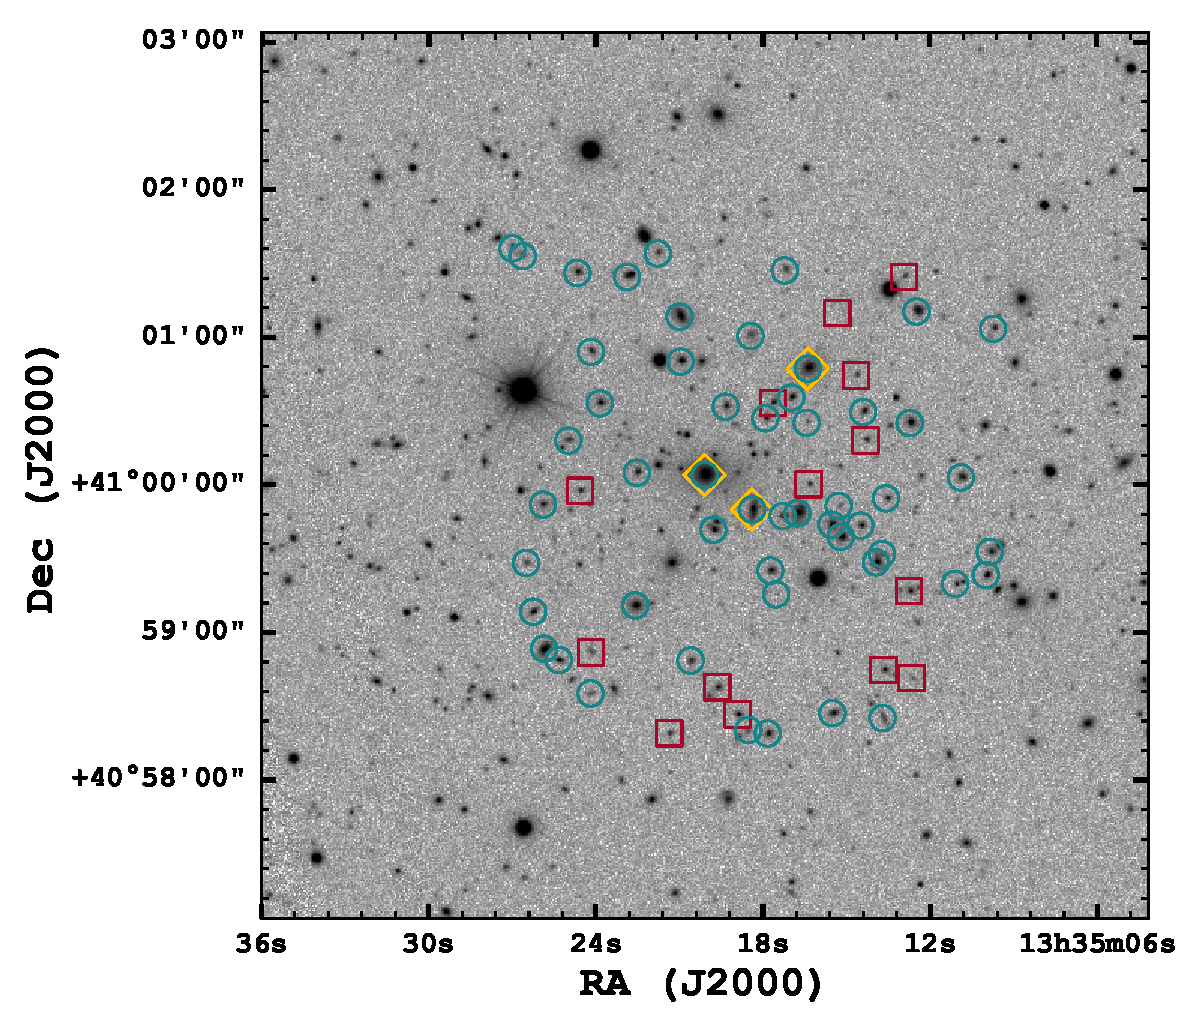
\includegraphics[width=0.5\textwidth]{./figures2/c203p83+41p0_mosaic.pdf}
}
\hfill
\subfloat{%
  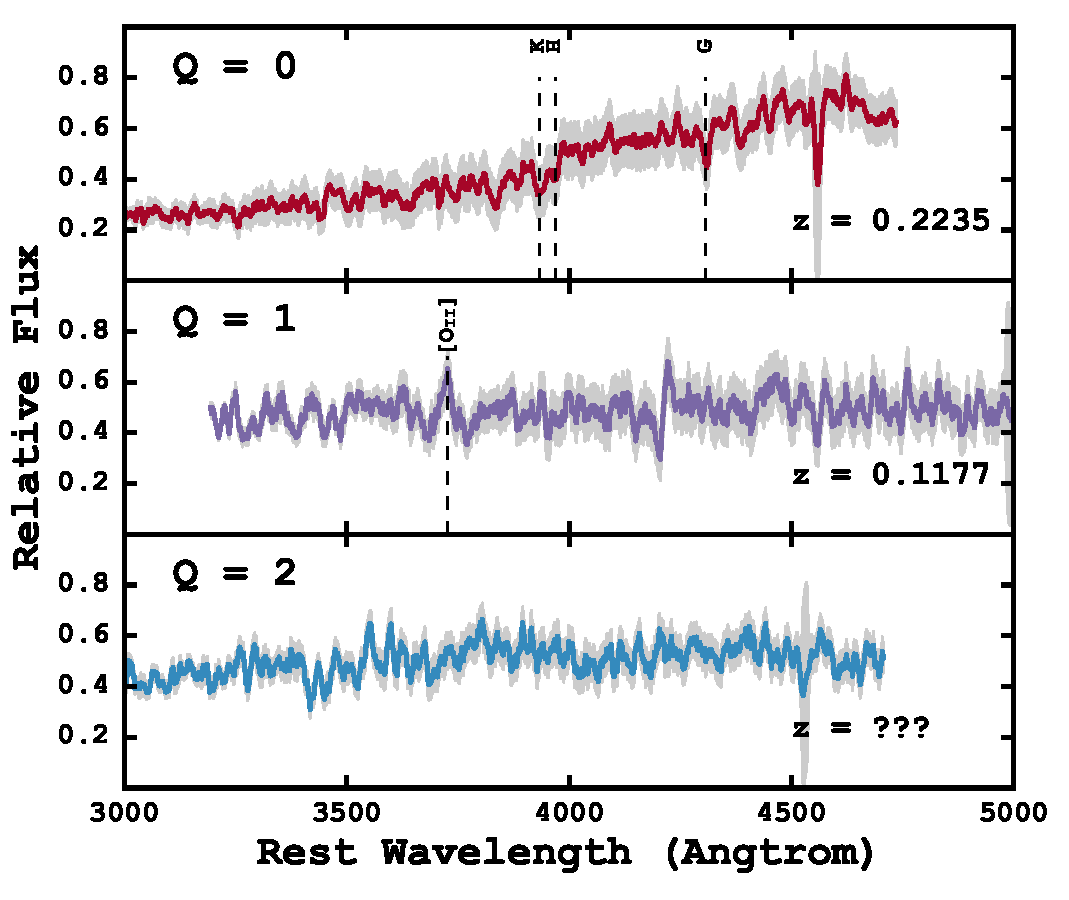
\includegraphics[width=0.5\textwidth]{./figures2/spectrum.pdf}
}
	\caption{SDSS \sdssr\ image of cluster c203p83+41p0 and spectra quality examples.}
    \emph{Left:} SDSS \sdssr\ image of cluster c203p83+41p0. The symbols show the position of observed galaxies. Blue circles indicate galaxies with $Q=0$ or $Q=1$ spectroscopic redshifts, red squares indicate galaxies where a redshift could not be reliably determined, and the orange diamond corresponds to galaxies with pre-existing redshifts from the SDSS. \textit{Right:} Example spectra, with major features identified, showing the three quality flags. $Q=0$ represents the best quality spectra and $Q=2$ the poorest quality. $Q=0$, and $Q=1$ are sufficient to measure galaxy redshifts. 
	\label{2fig:c203p83+41p0}
\end{figure}

% \begin{figure}
%      \begin{center}
%         \subfigure{\label{2fig:first}
%             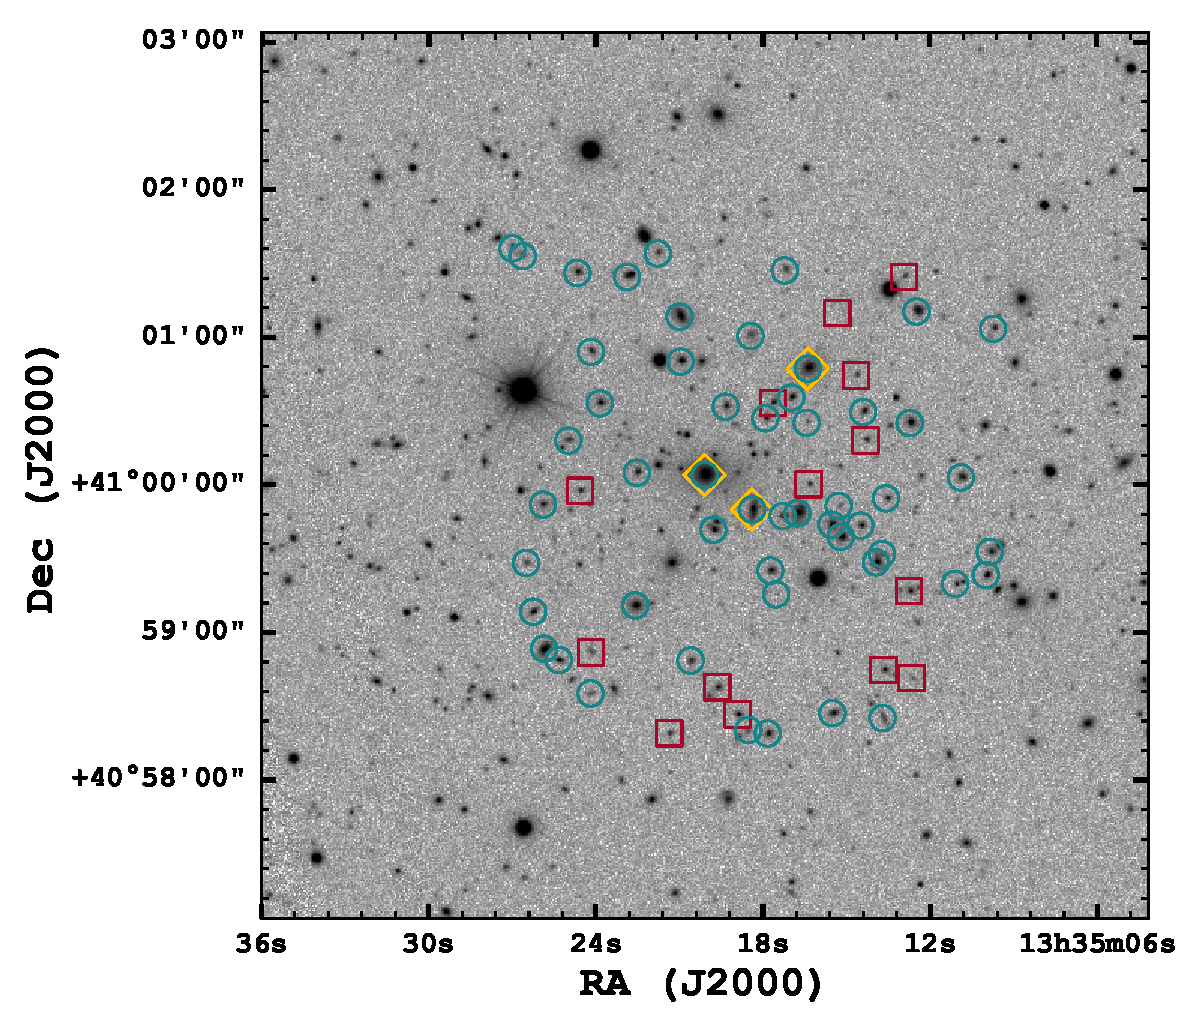
\includegraphics[width=\textwidth]{./figures2/c203p83+41p0_mosaic.pdf}
%         }
%         \subfigure{\label{2fig:second}
%            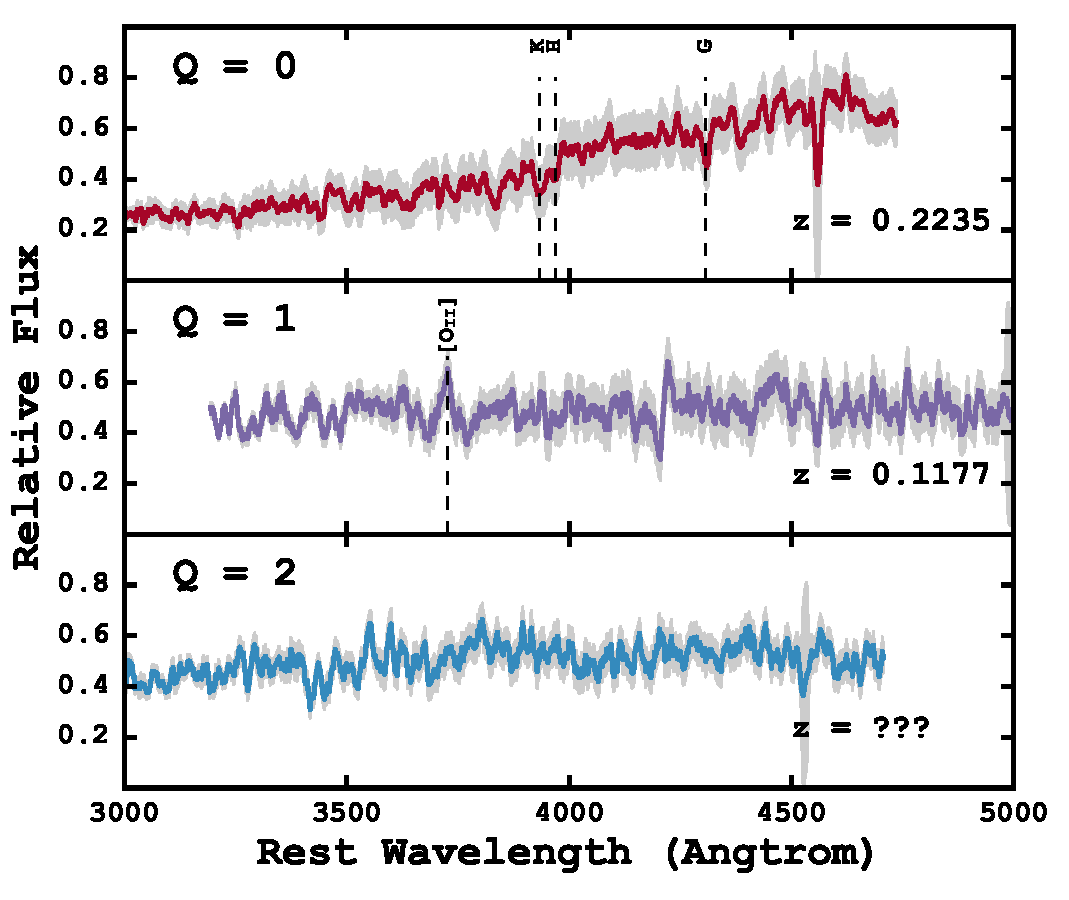
\includegraphics[width=\textwidth]{./figures2/spectrum.pdf}
%         }
%     \end{center}
%     \caption{SDSS \sdssr\ image of cluster c203p83+41p0. The symbols show the position of observed galaxies. Blue circles indicate galaxies with $Q=0$ or $Q=1$ spectroscopic redshifts, red squares indicate galaxies where a redshift could not be reliably determined, and the orange diamond corresponds to galaxies with pre-existing redshifts from the SDSS. \textit{Right:} Example spectra, with major features identified, showing the three quality flags. $Q=0$ represents the best quality spectra and $Q=2$ the poorest quality. $Q=0$, and $Q=1$ are sufficient to measure galaxy redshifts.}
% 	\label{2fig:c203p83+41p0}
% \end{figure}

After reducing all spectra we find an average residual mismatch in the wavelength solution of $\sigma_\lambda \sim 0.4$ \AAA\ or 24 \kms\ at 5000 \AAA. Fitting gaussians to each of the arc lines we find an average instrumental resolution of $\sim144$ \kms, and combining the two in quadrature gives a total instrumental resolution of $\sigma_{inst} = 146$ \kms, similar to that of other studies using the MS \citeeg{Murphy2011, Blanc2013}.

\section{Analysis}\label{2sec:analysis} 
The analysis of our reduced spectra occurs in two stages. First we derive individual redshifts using the observed galaxies, and then we work with the redshifts collectively to identify which galaxies likely belong to the galaxy cluster in question. This section outlines the steps required in each of those processes. 

Individual galaxy selection is done through cross matching the IFU fiber sky positions with galaxies selected from the SDSS. We select all galaxies brighter than 22 mag in \sdssg\ within $3'$ of the BCG in each cluster. For each galaxy we query the SDSS for photometry in all SDSS bands (\sdssu\sdssg\sdssr\sdssi\sdssz), photometric redshift, and any spectroscopic redshift. 

Because of the large number of fiber pointings, only fibers which overlap with SDSS sources are considered for redshift analysis. The left panel of Figure \ref{2fig:c203p83+41p0} shows cluster c203p83+41p0 with the SDSS detections and measured redshifts overlaid. Orange diamonds are galaxies with SDSS available redshifts. The blue circles and red squares correspond to galaxies where a redshift was and was not determined from the observed spectra. See Figure~\ref{2fig:montage} for similar representation of the remaining nine clusters.

\subsection{Redshift Catalog}\label{2sec:redshift catalog} 
A redshift solution is determined for each galaxy by cross-correlating \citep{Tonry1979} each of the spectra with six galaxy template spectra from the SDSS\footnote{http://classic.sdss.org/dr7/algorithms/spectemplates/index.html} using the \textsc{xcsao} task in the \textsc{iraf} \textsc{rvsao} package \citep{Kurtz1992, Kurtz1998}. For each galaxy we select the spectral template with the highest cross-correlation coefficient and visually inspect the fit. During visual inspection a ``Q'' or quality flag is assigned. High-confidence redshifts, clearly determined by at least two obvious features (such as the Ca H, K and E absorption features), receive $Q=0$, spectra with only a single strong feature (\eg, \hbox{[\ion{O}{ii}]} emission) are assigned $Q=1$ and redshifts resulting from enigmatic features are assigned $Q=2$. Figure~\ref{2fig:c203p83+41p0} shows representative example spectra for each of the $Q$ flags. For the determination of cluster properties we only consider $Q=0$ and $Q=1$ quality flags. 

\begin{figure}[t]
	\begin{center}
		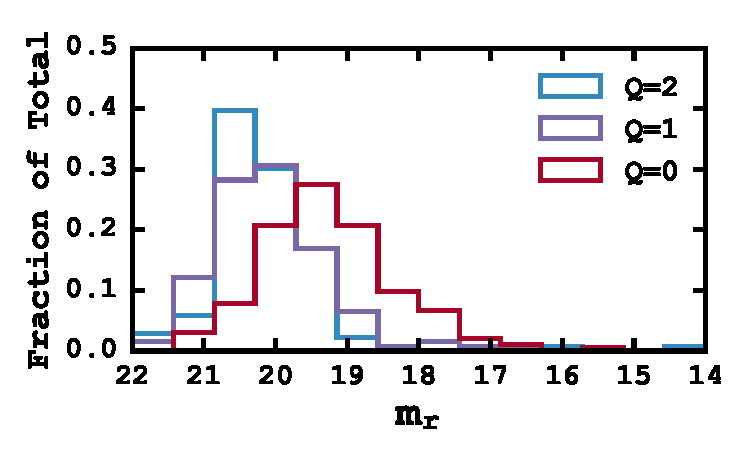
\includegraphics[width=0.6\textwidth]{figures2/redshiftHist.pdf}
	\end{center}
	 
	\caption{Redshift recovery fractions across all clusters.} 
	The bar heights represent the fraction of the total redshifts with the respective $Q$ value at a particular magnitude. For example, $\sim 40\%$ of the $Q=2$ redshifts have $m_r = 20.5-21$. We find a general decrease in redshift quality with increasing $m_r$. \label{2fig:redshiftHist} 
\end{figure}

Figure \ref{2fig:redshiftHist} shows the breakdown of $Q$ values for the redshifts across all clusters. We compute 447 redshifts, of which 44\% have $Q=0$, 27\% have $Q=1$ and 29\% have $Q=2$. We find a general decrease in $Q$ flag with increasing $m_r$. Approximately 30\% of the $Q=0$ redshifts correspond to galaxies with $19 < m_r <20$ whereas about 40\% $Q=2$ galaxies have $m_r = 20.5-21$.

\begin{landscape}
	\singlespace
	\begin{longtable}{ccccccccccc} 
	\caption{Spectroscopic redshifts for galaxies in c203p8+41p0 measured with the MS: Column 1: The telescope pointing; Column 2: The dither position; Column 3: The fiber number; Column 4: The right ascension of the galaxy; Column 5: The declination of the galaxy; Column 6: The the observed SDSS \sdssr\ magnitude; Column 7: The galaxy redshift; Column 8: The redshift $Q$ flag; Column 9: The galaxy membership information; Column 10: The clustercentric radial distance; Column 11: The LOSV of the galaxy with respect to the cluster. See the appendix for similar tables for the remaining nine clusters.}\\
	\hline
	tile & dither & fiber & RA (J2000) & DEC (J2000) & \sdssr\ (mag) & redshift & $Q$ & Member & R (Mpc) & LOSV (\kms) \\
	(1) & (2) & (3) & (4) & (5) & (6) & (7) & (8) & (9) & (10) & (11) \\
	\hline \hline
	\endfirsthead
	\multicolumn{4}{l}%
	{\tablename\ \thetable\ Continued} \\
	\hline
	tile & dither & fiber & RA (J2000) & DEC (J2000) & \sdssr\ (mag) & redshift & $Q$ & Member & R (Mpc) & LOSV (\kms) \\
	(1) & (2) & (3) & (4) & (5) & (6) & (7) & (8) & (9) & (10) & (11) \\
	\hline \hline
	\endhead
	NE & 1 & 14 & 13:35:27.004 & +41:01:36.20 & 20.47 & 0.2019$\pm{0.0003}$ & 1 & ... & 0.40 & -6945$\pm{146}$ \\
	NE & 1 & 111 & 13:35:24.177 & +41:00:54.16 & 20.10 & 0.1178$\pm{0.0001}$ & 1 & ... & 0.15 & -27397$\pm{63}$ \\
	NE & 1 & 154 & 13:35:23.853 & +41:00:33.19 & 19.28 & 0.2214$\pm{0.0002}$ & 0 & ... & 0.18 & -2214$\pm{83}$ \\
	NE & 2 & 6 & 13:35:21.777 & +41:01:34.15 & 20.38 & 0.1691$\pm{0.0002}$ & 1 & ... & 0.27 & -14929$\pm{102}$ \\
	NE & 2 & 14 & 13:35:26.632 & +41:01:33.06 & 20.95 & 0.0403$\pm{0.0003}$ & 0 & ... & 0.09 & -46214$\pm{131}$ \\
	NE & 2 & 63 & 13:35:20.998 & +41:01:08.49 & 17.90 & 0.2381$\pm{0.0001}$ & 0 & $\checkmark$ & 0.25 & 1849$\pm{49}$ \\
	NE & 3 & 22 & 13:35:22.879 & +41:01:24.60 & 19.76 & 0.2386$\pm{0.0003}$ & 0 & $\checkmark$ & 0.33 & 1961$\pm{131}$ \\
	NE & 3 & 25 & 13:35:24.669 & +41:01:26.21 & 19.54 & 0.1444$\pm{0.0001}$ & 0 & ... & 0.25 & -20924$\pm{58}$ \\
	NE & 3 & 73 & 13:35:18.447 & +41:01:00.60 & 19.63 & 0.0779$\pm{0.0001}$ & 0 & ... & 0.09 & -37080$\pm{29}$ \\
	NE & 3 & 106 & 13:35:20.957 & +41:00:50.19 & 18.83 & 0.2235$\pm{0.0002}$ & 0 & $\checkmark$ & 0.17 & -1691$\pm{78}$ \\
	NE & 3 & 147 & 13:35:19.341 & +41:00:31.82 & 19.48 & 0.2380$\pm{0.0001}$ & 0 & ... & 0.11 & 1822$\pm{73}$ \\
	NE & 3 & 185 & 13:35:24.990 & +41:00:18.06 & 20.51 & 0.1887$\pm{0.0002}$ & 1 & ... & 0.18 & -10169$\pm{83}$ \\
	NE & 3 & 206 & 13:35:20.095 & +41:00:04.12 & 16.39 & 0.2274$\pm{0.0001}$ & 1 & $\checkmark$ & 0.00 & -763$\pm{34}$ \\
	NE & 3 & 210 & 13:35:22.528 & +41:00:05.00 & 19.59 & 0.2242$\pm{0.0001}$ & 1 & $\checkmark$ & 0.10 & -1543$\pm{49}$ \\
	NW & 1 & 127 & 13:35:16.384 & +41:00:47.33 & 17.43 & 0.2377$\pm{0.0001}$ & 0 & $\checkmark$ & 0.23 & 1752$\pm{68}$ \\
	NW & 1 & 167 & 13:35:14.400 & +41:00:29.73 & 19.69 & 0.2333$\pm{0.0002}$ & 0 & $\checkmark$ & 0.26 & 690$\pm{117}$ \\
	NW & 2 & 27 & 13:35:17.216 & +41:01:27.25 & 20.21 & 0.1512$\pm{0.0002}$ & 0 & ... & 0.24 & -19279$\pm{117}$ \\
	NW & 2 & 63 & 13:35:12.486 & +41:01:10.57 & 18.84 & 0.1638$\pm{0.0001}$ & 0 & ... & 0.31 & -16210$\pm{44}$ \\
	NW & 2 & 73 & 13:35:09.729 & +41:01:03.49 & 20.00 & 0.2402$\pm{0.0001}$ & 1 & ... & 0.50 & 2367$\pm{58}$ \\
	NW & 2 & 165 & 13:35:12.728 & +41:00:25.16 & 18.74 & 0.2394$\pm{0.0001}$ & 0 & $\checkmark$ & 0.33 & 2155$\pm{58}$ \\
	NW & 2 & 171 & 13:35:16.434 & +41:00:25.31 & 21.68 & 0.1617$\pm{0.0002}$ & 1 & ... & 0.13 & -16728$\pm{121}$ \\
	NW & 2 & 173 & 13:35:17.911 & +41:00:27.16 & 19.49 & 0.1039$\pm{0.0002}$ & 0 & ... & 0.06 & -30763$\pm{107}$ \\
	NW & 2 & 220 & 13:35:10.891 & +41:00:03.07 & 19.45 & 0.2994$\pm{0.0002}$ & 0 & ... & 0.47 & 16739$\pm{102}$ \\
	NW & 2 & 239 & 13:35:13.582 & +40:59:54.58 & 20.24 & 0.2316$\pm{0.0002}$ & 1 & $\checkmark$ & 0.28 & 265$\pm{92}$ \\
	NW & 3 & 142 & 13:35:16.981 & +41:00:35.55 & 19.44 & 0.2233$\pm{0.0002}$ & 0 & $\checkmark$ & 0.17 & -1745$\pm{78}$ \\
	SE & 1 & 27 & 13:35:25.896 & +40:59:52.05 & 19.35 & 0.2295$\pm{0.0004}$ & 1 & $\checkmark$ & 0.25 & -238$\pm{170}$ \\
	SE & 1 & 46 & 13:35:19.779 & +40:59:41.85 & 18.73 & 0.2293$\pm{0.0002}$ & 0 & $\checkmark$ & 0.08 & -284$\pm{107}$ \\
	SE & 1 & 86 & 13:35:26.506 & +40:59:28.30 & 20.59 & 0.2255$\pm{0.0002}$ & 1 & $\checkmark$ & 0.29 & -1205$\pm{112}$ \\
	SE & 1 & 123 & 13:35:22.588 & +40:59:11.02 & 18.17 & 0.2307$\pm{0.0002}$ & 0 & $\checkmark$ & 0.22 & 44$\pm{102}$ \\
	SE & 1 & 129 & 13:35:26.254 & +40:59:08.50 & 19.42 & 0.1282$\pm{0.0002}$ & 0 & ... & 0.20 & -24863$\pm{107}$ \\
	SE & 2 & 164 & 13:35:20.600 & +40:58:48.65 & 20.02 & 0.2938$\pm{0.0001}$ & 0 & ... & 0.33 & 15369$\pm{53}$ \\
	SE & 3 & 157 & 13:35:25.857 & +40:58:53.46 & 18.31 & 0.1701$\pm{0.0001}$ & 0 & ... & 0.28 & -14684$\pm{29}$ \\
	SE & 3 & 171 & 13:35:25.332 & +40:58:48.88 & 19.49 & 0.2400$\pm{0.0003}$ & 0 & ... & 0.36 & 2296$\pm{126}$ \\
	SE & 3 & 198 & 13:35:24.191 & +40:58:35.23 & 20.83 & 0.1177$\pm{0.0002}$ & 1 & ... & 0.21 & -27419$\pm{87}$ \\
	SW & 1 & 41 & 13:35:17.295 & +40:59:47.40 & 19.87 & 0.2231$\pm{0.0002}$ & 0 & ... & 0.13 & -1808$\pm{107}$ \\
	SW & 1 & 114 & 13:35:17.529 & +40:59:15.55 & 20.60 & 0.2493$\pm{0.0003}$ & 1 & ... & 0.22 & 4561$\pm{156}$ \\
	SW & 1 & 224 & 13:35:13.709 & +40:58:25.25 & 20.03 & 0.1276$\pm{0.0003}$ & 0 & ... & 0.28 & -25006$\pm{126}$ \\
	SW & 1 & 227 & 13:35:15.509 & +40:58:27.26 & 19.27 & 0.2328$\pm{0.0002}$ & 0 & $\checkmark$ & 0.41 & 559$\pm{83}$ \\
	SW & 1 & 245 & 13:35:17.832 & +40:58:19.02 & 19.29 & 0.2211$\pm{0.0003}$ & 1 & ... & 0.39 & -2275$\pm{136}$ \\
	SW & 1 & 246 & 13:35:18.529 & +40:58:20.43 & 21.31 & 0.1970$\pm{0.0002}$ & 1 & ... & 0.34 & -8140$\pm{117}$ \\
	SW & 2 & 24 & 13:35:15.282 & +40:59:51.52 & 21.29 & 0.2225$\pm{0.0002}$ & 1 & $\checkmark$ & 0.20 & -1934$\pm{97}$ \\
	SW & 2 & 29 & 13:35:18.391 & +40:59:50.06 & 18.17 & 0.2405$\pm{0.0001}$ & 0 & ... & 0.09 & 2440$\pm{44}$ \\
	SW & 2 & 39 & 13:35:15.539 & +40:59:43.86 & 18.73 & 0.2263$\pm{0.0002}$ & 0 & $\checkmark$ & 0.20 & -1023$\pm{107}$ \\
	SW & 2 & 53 & 13:35:15.211 & +40:59:38.90 & 18.73 & 0.2412$\pm{0.0001}$ & 0 & $\checkmark$ & 0.23 & 2593$\pm{58}$ \\
	SW & 2 & 59 & 13:35:09.857 & +40:59:32.82 & 19.83 & 0.2334$\pm{0.0002}$ & 1 & $\checkmark$ & 0.45 & 697$\pm{107}$ \\
	SW & 2 & 65 & 13:35:13.725 & +40:59:31.94 & 20.58 & 0.3156$\pm{0.0003}$ & 0 & ... & 0.37 & 20688$\pm{156}$ \\
	SW & 2 & 86 & 13:35:17.737 & +40:59:25.25 & 19.71 & 0.2236$\pm{0.0002}$ & 0 & $\checkmark$ & 0.17 & -1684$\pm{78}$ \\
	SW & 2 & 90 & 13:35:11.098 & +40:59:19.79 & 20.41 & 0.2354$\pm{0.0002}$ & 0 & $\checkmark$ & 0.42 & 1195$\pm{97}$ \\
	SW & 3 & 26 & 13:35:16.763 & +40:59:48.52 & 17.94 & 0.2250$\pm{0.0001}$ & 0 & $\checkmark$ & 0.15 & -1334$\pm{34}$ \\
	SW & 3 & 37 & 13:35:14.503 & +40:59:43.50 & 19.79 & 0.2428$\pm{0.0002}$ & 0 & $\checkmark$ & 0.26 & 2979$\pm{107}$ \\
	SW & 3 & 65 & 13:35:13.944 & +40:59:28.57 & 18.60 & 0.2362$\pm{0.0001}$ & 0 & $\checkmark$ & 0.29 & 1385$\pm{58}$ \\
	SW & 3 & 73 & 13:35:10.002 & +40:59:23.42 & 19.52 & 0.2307$\pm{0.0001}$ & 0 & $\checkmark$ & 0.45 & 39$\pm{73}$ \\
	\hline 
	\label{2tbl:c203p83+41p0} 
	\end{longtable}
\end{landscape}


\textsc{xcsao} reports errors on the cross-correlation redshift. Previous work \citeeg{Quintana2000, Sifon2015a} show the cross-correlation velocity uncertainties by up to a factor of two. We report our redshift uncertainties as twice the uncertainty estimated by \textsc{xcsao}.

Redshift information, with $Q=0$ or $Q=1$ spectra, for each galaxy are given in Table~\ref{2tbl:c203p83+41p0}. The right panel of Figure~\ref{2fig:c203p83+41p0} shows selected spectra from cluster c203p83+41p0 with corresponding best fitting SDSS template. See the appendix for similar examples from the remaining nine clusters.

\subsection{Cluster Membership}\label{2sec:cluster membership} 
The determination of cluster membership begins with the calculation of the cluster central redshift. This serves as a zero-point from which all other galaxies will be compared. Therefore, the accurate determination of the cluster redshift ($z_c$) is crucial to the reliability of all following measurements. An incorrect cluster redshift introduces errors into the measured line of sight velocity (LOSV) and corresponding dispersion, which, in turn, contributes to errors associated with dynamical mass and radius. 

In simple terms, the cluster redshift is the mean of the redshifts of all galaxies associated with the cluster. However, because the standard mean can be quite sensitive to outliers or otherwise contaminated data, we require a more resistant statistic, and turn to the biweight location estimator \citep{Beers1990} which provides improved performance. The biweight location does not give us the freedom to use all galaxies measured but provides protection against a small number of interlopers. Therefore, the process of determining $z_c$ and the cluster membership are linked. We begin with the nominal $z_c$ (see Table~\ref{2tbl:targets}) and apply and initial velocity cut of 5000 \kms\ to remove any foreground or background galaxies. Then, using the membership determination techniques described below we determine the member galaxies from which a new $z_c$ is calculated. The entire process is repeated until convergence, usually within a single iteration. The cluster central redshift and associated 68\% uncertainties, derived from bootstrap shuffling, are given in Table~\ref{2tbl: derived parameters}.

To reject the galaxies not associated with the targeted cluster, we employ two methods. For clusters with 20 or more $Q=0$ or $Q=1$ redshifts we use the ``shifting gapper'' method of \citeeg{Fadda1996, Crawford2014}, which combines both the positional and velocity information. Galaxies are first sorted by their radial separation from the cluster center (See Table~\ref{2tbl:targets}) and binned into radial bins of at least 10 members. Once in the radial bins, the galaxies are sorted by the LOSV, 
\begin{equation}
	LOSV = c\frac{(z-z_{c})}{(1+z_{c})} 
\end{equation}
where $c$ is the speed of light in \kms, $z$ is the redshift of the individual galaxy and $z_{c}$ is the redshift of the cluster. Any galaxy with a LOSV greater than 1000 \kms of a neighboring galaxy (the velocity ``gap'') is rejected as an interloper. The procedure repeats until the number of galaxies stabilizes in the bin. Once the members have been identified we recompute $z_c$, LOSVs, and begin the membership selection again. This entire process is repeated until the number of member galaxies stabilizes. 

For galaxy clusters with fewer than 20 $Q=0$ or $Q=1$ redshifts we employ the general of membership determination method outlined in \cite{Wilman2005, Connelly2012}. We assume an initial velocity dispersion, $\sigma(v)$, of 500$(1+z)$\kms\ and apply both redshift and spatial limits given by: 
\begin{equation}
	\delta(z)_{max} = 2 \sigma(v)/c 
\end{equation}
and 
\begin{equation}
	\delta(r)_{max} = \frac{c\times\delta(z)_{max}}{bH(z)} 
\end{equation}
where $b=9.5$ is the aspect ratio, $H(z) = H_0 E(z)$ and $E(z) = \sqrt{\Omega_m(1+z^3)+\Omega_{\Lambda}}$. We select all galaxies with $|z-z_c| < \delta(z)_{max}$ and radial separation, $R$, $<\delta(r)_{max}$. During each step, we update both the $z_c$ and $\sigma(v)$ using the identified members and this process is repeated until the number of member galaxies converges. 

To calculate the velocity dispersion in this membership determination method, we use the gapper estimator \citep{Beers1990} which provides accurate dispersions for groups as small as five members \citep{Hou2009}. It is given by 
\begin{equation}
	\sigma_g = \frac{\sqrt{\pi}}{n(n-1)} \sum_{i=1}^{n-1} w_i g_i
\end{equation}
where the weights are $w_i = i(n-i)$ and $g_i = x_{i+1} - x_i$ are the gaps between ordered pairs of LOSVs. The dispersion estimate is corrected by $1.135$ to account for the $2\sigma$ redshift space cut applied during membership determination. We follow this method for the calculation of the dispersion for consistency in member determination only. The final velocity dispersion of each cluster is determined din the following subsection.

Membership information for the galaxies observed in and around cluster c203p83+41p0 is given in Column 9 of Table~\ref{2tbl:c203p83+41p0}. See the appendix for the membership of the other observed clusters.

\subsection{Line-of-Sight Velocity Dispersion}\label{2sec:LOSVD}
To compute the line-of-sight velocity dispersion (LOSVD) of each cluster we follow the maximum likelihood method of \cite{Walker2006}. We assume that the each galaxy is drawn from a Gaussian distribution centered on the mean cluster velocity and we maximize the log of the product of each cluster member's individual Gaussian probabilities (their Eq. 8):
\begin{equation}
  \label{2eq:log}
\ln(p)=-\frac{1}{2}\sum_{i=1}^{N}\ln(\sigma_i^2+\sigma_p^2)-\frac{1}{2}\sum_{i=1}^N\frac{(v_i-\langle u \rangle)^2}{(\sigma_i^2+\sigma_p^2)}-\frac{N}{2}\ln(2\pi).
\end{equation}
where $\sigma_p$, $\langle\mu\rangle$, and $\sigma_i$ is the LOSVD, the average radial velocity and the error on the individual LOSVs respectively. To maximize the probability, we use {\sc emcee}\footnote{http://dan.iel.fm/emcee/current/} \citep{Foreman-Mackey2013}, a Monte Carlo Markov Chain (MCMC) sampler, based on affine-invariant ensemble sampler (see \citealt{Goodman2010} for details on affine-invariant samplers). We set priors on $\langle\mu\rangle$, and $\sigma_p$ by requiring that $\langle\mu\rangle$ lies between the maximum and minimum LOSV and that $\sigma_p$ be positive and less than $1400$ \kms which corresponds approximately to a $10^{16}$ \Msol\ cluster at $z=0$, larger than any expected cluster mass in our sample. We draw twenty thousand samples from the posterior probability distribution and report a measured LOSVD as the median value of the posterior probability distribution with 68\% error bars defined as the square root of the second moment of the same distribution.

\subsection{Power Law Estimates of Cluster Mass}
We adopt the scaling relation of \cite{Munari2013} to estimate cluster masses based solely on their LOSVD. The scaling relation is based on the work of \cite{Evrard2008} and has the form: 
\begin{equation}\label{2eq:power law}
	M_{200c} = \frac{10^{15}}{h(z)} \bigg{(}\frac{\sigma_{1D}}{A_{1D}} \bigg{)}^{1/\alpha} \Msol 
\end{equation}
where $A_{1D} =1177\pm4.2$ \kms, $\alpha = 0.634\pm0.0021$, $h(z) = H(z)/100$, and $\sigma_{1D}$ is the LOSVD. The relation is calibrated through a cosmological simulation using galaxies (instead of dark matter particles or subhalos) as the tracers of LOSVD. This choice of tracer results in dynamical masses which are $16-26\%$ lower \citeeg{Kirk2015, Sifon2015a} than masses obtained through the scaling relation of \cite{Evrard2008}, which has been calibrated using dark matter particles alone. This is due dynamical effects which act upon the galaxies but not the dark matter particles.

\section{Machine Learning Methods}\label{2sec:ML methods}
The goal of this section is to describe the methods used to create a suitable training set for a machine learning (ML) method and to then predict the dynamical masses of the ten clusters in our sample. In order to accomplish this, we must first assign $Q$ flags to a mock galaxy catalog which, as best possible, accurately reflect the actual observations described previously. This will allow us to construct a catalog which contains galaxies which closely resemble the galaxies observed with the MS.

We begin the discussion with a brief introduction to supervised ML methods and a discussion about the creation of the mock galaxy catalogs used in this analysis. We then discuss the process used to assign the $Q$ flags and conclude with an overview of the method we use to make cluster mass predictions.

\subsection{Supervised Machine Learning}
ML is a subfield of computer science which provides tools to give computers the ability to infer the relationship between known variables without that relationship being explicitly programed. Supervised ML provides the algorithm with a set of known inputs, ``features'' in ML speak, and a set of desired outputs or ``targets.'' The relationship between the features and targets is determined through the use of a training set. The ML algorithm is first provided with both the features and targeted which it uses to infer their relationship, then it is given a new set of features which it uses to predict the desired targets. 

Because there are many different ML algorithms the initial training set is often broken into a \emph{training} and \emph{testing} set \citeeg{Ripley2007, Xu2013, Ntampaka2015, Ntampaka2015a, Acquaviva2016}. For both sets the desired targets are known, so they can be used to both train the ML method and to test how well it predicts the desired targets. The performance achieved can be used to select the best ML method. Once an algorithm is selected we can attempt to optimize the model's input parameters (often called hyper-parameters) by further splitting the training sample into a cross-validation (CV) set. We use 5-fold CV throughout.

Just as in \citetalias{Boada2016}, we rely on an ensemble ML method \citeeg{Caruana2006} where we use many estimators and then combine them at the end to make the best possible prediction. The combination of estimators come in two flavors. Averaging methods average the final estimates together into a single prediction, and boosting estimators which seek to boost the predictive power by combining weak estimates at each step in the learning process.

A forest of randomized decision trees (or random forest; RF; \citealt{Ho1995, Ho1998}) is a type of ensemble method where the trees can be visualized as flow chart. The path through the flow chart (the trees) is decided by the values of the training features at each fork. RF use a random subset of the train data to decide which fork should be followed. The final prediction is the mean of each tree's final value. We use RF methods implemented in the {\sc Scikit-Learn} \citep{Pedregosa2012} Python library.

\subsubsection{The Buzzard Catalog}
We require a catalog which provides both the observable features and desired targets in order to train our ML method. The ``Buzzard'' mock galaxy catalog contains 238 million galaxies with \sdssr\ mag $< 29$ and $z \leq 8.7$. The galaxies are located in a 398.49 \degsq\ portion of the sky and their luminosities are derived from a combination of Sub-halo Abundance Matching (SHAM; \citealt{Reddick2013}) and Adding Density Dependent Spectral Energy Distributions (ADDSED). The galaxies are assigned to the dark matter halos identified by the {\sc ROCKSTAR} halo finder \citep{Behroozi2013}. The catalogs assume the following cosmological parameters: $\Omega_\Lambda = 0.714$, $\Omega_M = 0.286$, $\sigma_8 = 0.82$ and $H_0= 70$ \kms \mpc. See \citetalias{Boada2016} for a more thorough description of the process used to create the catalogs.

\subsection{ML Based Observations}
In order to create a mock dataset which resembles our actual observations we first rely on the RF method as a classifier. The goal is to assign each galaxy in the Buzzard catalog a $Q$ flag of either 0, 1 or 2 based on their observed magitudes in the five SDSS filters, \sdssu\sdssg\sdssr\sdssi\sdssz, the ten combinations of possible colors, and the square of those colors. \cite{Acquaviva2016} uses a similar feature set to predict the metallicity of SDSS galaxies with good effect. 

The RF classifier is tasked with learning which combinations of magnitudes and colors best separates the three possible $Q$ flags and to assign each Buzzard galaxy into one of those classes. The classifier is trained using the redshift catalog derived from our cluster observations (Section \ref{2sec:redshift catalog}), and the 447 observations are split into a training, CV and test sample. We use the training set to train the ML method, the CV set to tune the model hyper-parameters and the test sample to verify how well our model classifies each galaxy. We also perform recursive feature elimination to remove features which contribute very little to the classification.

We compute two statistics to evaluate how well our model classifies the galaxies, the recall and the precision. The recall is the number predicted compared to the true number of classifications, $N_{pred}/N_{true}$. The precision is the number of correct predictions compared to the total number of predictions for each class, $N_{corr}/N_{pred}$. In both cases the metrics range from zero to one, and higher numbers are better. For our optimized RF classifier we achieve overall recall and precision of $\sim60\%$. For the individual classes ($Q$ flags), the RF classifier performs significantly better when classifying $Q=0$ and $Q=2$ galaxies, with recall rates well above 70\%. The $Q=1$ training galaxies have significant overlap between $Q=0$ and $Q=2$ (see Figure \ref{2fig:redshiftHist}) which leads to a recall for $Q=1$ galaxies of only $\sim20\%$. 

This is a difficult problem. Figure~\ref{2fig:redshiftHist} shows there is significant overlap between the $Q$ flags. In our testing, we find no combination of features which wholly separates the $Q$ flags, providing a high level of confusion for the RF. We find similar levels of recall and precision for other ML classification methods besides RF.

\begin{figure}[t]
	\begin{center}
		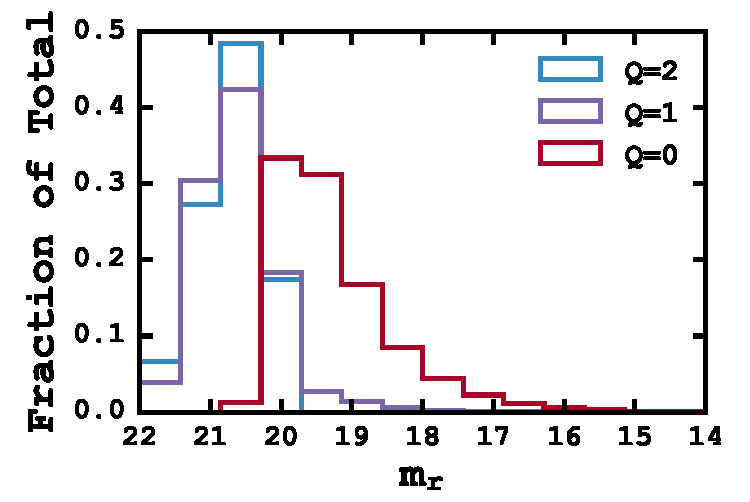
\includegraphics[width=0.6\textwidth]{figures2/buzzardQHist.pdf}
	\end{center}
	\caption{Quality flag ($Q$) assignments for the 2.7 million Buzzard catalog galaxies with $\sdssg< 22$ mag.} 
	The bar heights represent the fraction of the total redshifts with the respective $Q$ value at a particular magnitude. The distributions resemble the actual observations in Figure \ref{2fig:redshiftHist}. See the text for a detailed explanation of the classification process. \label{2fig:buzzardHist} 
\end{figure}

We assign each galaxy in the Buzzard catalog with $z<0.5$ and $\sdssg< 22$ mag a $Q$ flag using the optimized RF classifier trained with all 447 observations. Figure \ref{2fig:buzzardHist} shows the $Q$ flag distribution as a function of \sdssr\ magnitude. The total distribution of the 2.7 million $Q$ flags is 45.6\% $Q=0$, 24.7\% $Q=1$, and 29.6\% $Q=2$. This distribution closely resembles the fractions of the actual observations with some $Q=1$ galaxies misclassified as $Q=0$. Because we use galaxies with either $Q=0$ or $Q=1$ this is does not significantly bias our analysis.

\subsection{ML Based Cluster Masses}\label{2sec:ML based cluster masses}
We use the ``observed'' ($Q=0$ and $Q=1$) galaxies created in the previous subsection to construct total mass distributions of the mock clusters. For this task we again use a RF, not as a classifier but as a regressor, which predicts a cluster mass given a set of input features, such as the observed LOSVD and redshift. Similarly to our classification methods, we create an optimized ML method by splitting the Buzzard catalogs into a training, CV, and testing set. 

Because the cluster masses presented with this method are predictions based on the feature data, any uncertainties quoted by this method are prediction intervals not confidence intervals. Prediction intervals are an estimate of the interval encompassing future observations, with a given probability. Confidence intervals, on the other hand, describe the different moments of a population. The prediction intervals are unique to each prediction, and are often based on the underlying assumption of normally distributed residuals. RF estimators do not assume normally distributed residuals, and thus, require special treatment.  

The prediction intervals for our RF estimator as based on the method of quantile regression forests \citep{Meinshausen2006}. The basic principle is that we record all response variables (the predictions), not simply the mean. This allows us to give the prediction as the full conditional probability distribution of all possible predictions. For brevity, we quote predicted masses as the median prediction and the 68\% prediction interval as the square root of the second moment of the full conditional probability distribution.

\subsection{The Importance of Training Features}\label{2sec: training features}
\begin{figure}[t]
	\begin{center}
		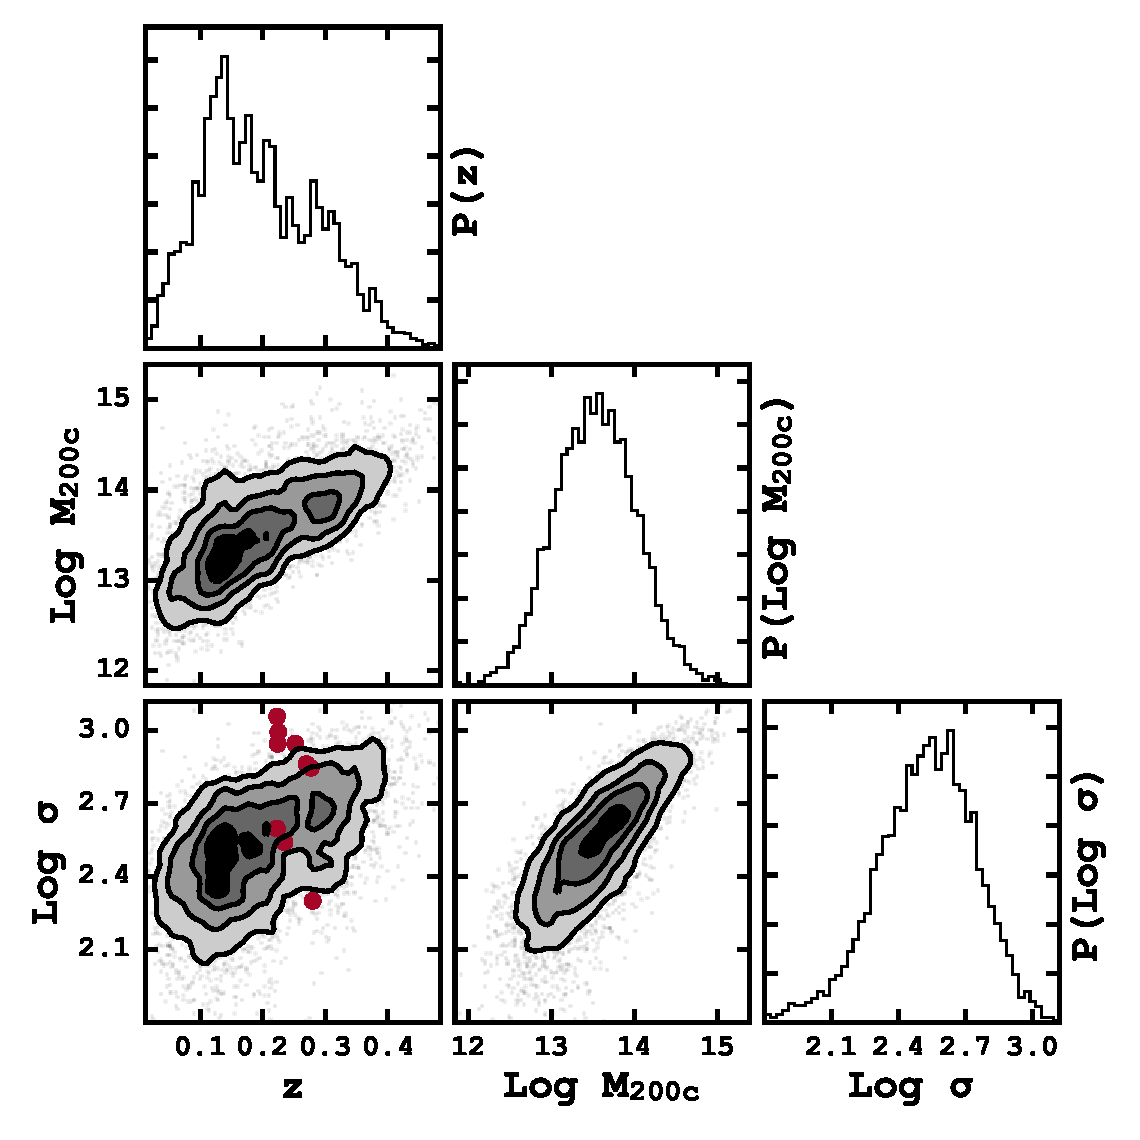
\includegraphics[width=0.6\textwidth]{figures2/buzzardCorner.pdf}
	\end{center}
	\caption{Corner plot of the \emph{training} data with features $\sigma$ and $z$.} 
	The corner plots shows all of the one and two dimensional posterior probability distributions used to determine the correct cluster mass. The colored circles show the position in the Log $\sigma$-redshift plane of the ten clusters in this sample.
	\label{2fig:buzzardCorner}
\end{figure}

The data used to train our ML algorithm is critical to the success of the method. We require training data which is broad enough to expose the ML method to a wide enough range of cluster parameters as not to influence the final outcome. If we use training data which include only galaxy clusters with $M < 10^{13}$ \Msol, for example, then it would not be able to correctly identify clusters with higher masses. 

The features of our training sample can be selected such that it does not bias the final predictions in an expected way. Figure~\ref{2fig:buzzardCorner} shows the $\sigma$ and $z$ features of the training sample from the Buzzard catalogs. The large red circles indicate the observed positions of our ten clusters in relation to the training data. Immediately noticeable, is that our observed clusters occupy a narrow redshift range ($0.2< z <0.3$). We also notice that seven of the ten clusters sit at the top edge of the training data in the $z$-Log $\sigma$ plane. Because the observed clusters are separate from the training data, the accuracy of the predictions of the cluster masses will be diminished. 

Effectively, the narrow redshift range where our observed clusters lie reduces the predicted cluster mass of the high mass clusters. This can be seen by moving the red points in Figure~\ref{2fig:buzzardCorner} up into the $z$-Log $M_{200c}$ plane where very few clusters with $0.2< z <0.3$ have masses above $10^{14}$ \Msol.

To combat the effect of cluster mass under-prediction, we make two critical changes from our method presented in \citetalias{Boada2016}. First, instead of using the membership information provided by the Buzzard catalogs we observe the clusters much in the same way we have with our actual observations. We select all galaxies within $2\farcm3$ around the center of each cluster (see Figure~\ref{2fig:tiles} for an illustration), and determine the cluster membership using the methods described in Section~\ref{2sec:cluster membership}. This serves to broaden the LOSVD distribution of the training data as interloping galaxies are certainly to be erroneously included.

Secondly, we exclude the redshift information from the training features when predicting the cluster masses. This has the effect of flattening the HMF, allowing for high mass clusters to exist at all redshifts. 

\section{Results and Discussion}\label{2sec:results}
The goal of this work to perform a practical test of some of the potential applications of a HETDEX-like survey to cluster science. Here, we present the predicted total masses of our ten clusters and estimate the absolute scale and scatter of a richness-mass relation based on those cluster masses. Because the accuracy of the predicted cluster masses is paramount to a well constrained richness-mass relation, we combine our results presentation with a discussion on their accuracy. 
 
\subsection{Cluster Masses}
\begin{figure}
	\centering 
	\includegraphics[height=0.75\textheight]{figures2/MLcomparison_shifty.pdf}
	\caption{ML based cluster mass predictions} 
	Mass predictions for the power law scaling relation (Equation~\ref{2eq:power law}) and the ML based technique with different input features as a function of true cluster mass. The bottom row of panels shows the fractional error (Equation~\ref{2eq: fractional error}) also as a function of true cluster mass. The solid black line shows the 1:1 relation. The solid, colored line is the median predicted mass for the targeted observing, and the colored, dashed line is the median recovered mass for the HETDEX-like observations. The shaded regions represent the 68\% scatter around the median values. \label{2fig: ML comparison} 
\end{figure}

In \citetalias{Boada2016} we found that the ML based method with the LOSVD ($\sigma$), redshift ($z$) and number of galaxies observed ($N_{gal}$) showed both the smallest bias and scatter over the largest range of cluster masses. This worked well because the training data were selected from a volume of similar size to the survey in question. As discussed previously, we modify our analysis slightly and use the power law based approach (Eqn.~\ref{2eq:power law}) and the $\mathrm{ML}_{\sigma, N_{gal}}$ method to estimate the masses of our ten clusters.

The prediction process uses two steps. Firstly, we use a method to predict the individual masses and secondly we correct those masses based on the results of the training data. The upper panel of Figure~\ref{2fig: ML comparison} show the cluster mass predictions for the Buzzard catalog clusters using the power law and $\mathrm{ML}_{\sigma, N_{gal}}$ approaches. The black diagonal line shows the perfect 1:1 relation. The lower panel of Figure~\ref{2fig: ML comparison} show the fractional error 
\begin{equation}\label{2eq: fractional error}
	\epsilon = (M_{pred} - M_{200c})/M_{200c}
\end{equation}
as a function of true cluster mass.

Using the predicted cluster masses for the Buzzard catalog we can quantify the amount of bias, and the scatter about that bias for different bins of predicted cluster mass. The bias is correctable by simply shifting our predicted cluster mass up or down by the appropriate amount. The scatter estimates the overall mass scale uncertainty in each bin of predicted cluster mass. We report the uncertainties in our cluster mass estimates as the sum in quadrature of the either confidence interval of the power law method or the prediction interval from the ML method and the mass scale uncertainty discussed here. \editorial{The problem with this is that we are about to talk about how the training data isn't like the SDSS data. So why are we going to correct our masses, PL or ML, using this data. If we aren't going to correct with it, then why go through all that exercise? We could only correct in the $10^{13}-10^{14}$ region where we have lots of clusters.}

\begin{landscape}
	\begin{table}
		\centering 
		\caption{Summary of derived cluster parameters: Column 1: The cluster name; Column 2: The number of SDSS sources observed; Column 3: The number of $Q=0(1)$ sources; Column 4: The number of member galaxies; Column 5: The redshift of the cluster; Columns 6: The LOSVD; Column 7: The power law predicted cluster mass; Column 8: The ML predicted cluster mass.} 
		\begin{tabular}
			{lccccccc} \hline Cluster & Sources & Q=0 (1) & Members & $z_{c}$ & $\sigma$ (\kms) & Log $M_{pred}$/\Msol & Log $M_{pred}$/\Msol \\
			(1) & (2) & (3) & (4) & (5) & (6) & (7) & (8) \\
			\hline \hline 
			c16p23+0p06 & 41 & 10 (10) & 15 & 0.2727$\pm{0.003}$ & 1194$\pm{135}$ & 15.11$\pm{0.14}$ & 14.58$\pm{0.27}$ \\
			c203p83+41p0 & 67 & 35 (17) & 25 & 0.2310$\pm{0.002}$ & 1314$\pm{91}$ & 15.24$\pm{0.08}$ & 14.71$\pm{0.47}$ \\
			c210p27+2p87 & 67 & 14 (30) & 16 & 0.2543$\pm{0.003}$ & 1295$\pm{115}$ & 15.22$\pm{0.11}$ & 14.55$\pm{0.45}$ \\
			c234p2+24p4 & 37 & 14 (14) & 11 & 0.2255$\pm{0.003}$ & 932$\pm{189}$ & 14.83$\pm{0.24}$ & 14.21$\pm{0.16}$ \\
			c250p08+46p7 & 61 & 36 (14) & 32 & 0.2274$\pm{0.002}$ & 1183$\pm{121}$ & 15.11$\pm{0.12}$ & 14.96$\pm{0.23}$ \\
			c260p61+32p13 & 61 & 26 (18) & 23 & 0.2260$\pm{0.002}$ & 1044$\pm{154}$ & 14.97$\pm{0.18}$ & 14.54$\pm{0.14}$ \\
			c319p70+0p56 & 45 & 21 (8) & 18 & 0.2750$\pm{0.003}$ & 820$\pm{148}$ & 14.67$\pm{0.22}$ & 14.30$\pm{0.12}$ \\
			c328p33+0p19 & 28 & 19 (2) & 16 & 0.2167$\pm{0.003}$ & 547$\pm{124}$ & 14.20$\pm{0.27}$ & 14.04$\pm{0.09}$ \\
			XMMXCSJ124425.9+164758.0 & 25 & 11 (8) & 6 & 0.2316$\pm{0.003}$ & 375$\pm{191}$ & 13.75$\pm{0.61}$ & 13.60$\pm{0.14}$ \\
			XMMXCSJ125650.2+254803.2 & 15 & 8 (3) & 3 & 0.2821$\pm{0.006}$ & 372$\pm{258}$ & 13.72$\pm{0.83}$ & 13.52$\pm{0.13}$ \\
			\hline 
		\end{tabular}
		\label{2tbl: derived parameters} 
	\end{table}
\end{landscape}


Table~\ref{2tbl: derived parameters} presents a summary of the derived parameters for each cluster. We include the LOSVD, the estimated cluster redshift, and the number of member galaxies observed. We provide two predicted cluster masses, the power law based cluster mass and the $ML_{\sigma, N_{gal}}$ predicted cluster mass. We discuss the accuracy of both of these predictions in the following subsections.

\subsection{Cluster Mass Accuracy}
Unlike our simulated galaxies in the Buzzard catalogs, we do not know the true cluster mass for our ten observed clusters. Fortunately, seven of the ten have other measurements from the literature. \cite{Sifon2015} report total cluster masses for four of our clusters. One has a reported LOSVD measurement and two have X-ray temperature measurements. We first compare our power law based cluster mass estimates to other estimates from the literature, and secondly we comment on the ML approach of predicting cluster masses.

\subsubsection{High Mass Clusters}
Total mass estimates for the four highest mass clusters are also reported by \cite{Sifon2015}. Using targeted spectra obtained with the Canada-France-Hawaii Telescope, they measure a LOSVD for each cluster. They convert the LOSVD into a dynamical cluster mass using the power law scaling relation of \cite{Evrard2008} (which is the basis of our Equation~\ref{2eq:power law}) and estimate the uncertainties using jackknife resampling. 

Mass estimates for three of the four clusters overlap within the $1\sigma$ error estimates, but the fourth cluster, c210p27+2p87 (Abell 1835), differs by almost a decade. c210p27+2p87 is a relatively well studied cluster, providing several cluster mass estimates. \cite{Hoekstra2012} report a LOSVD for c210p27+2p87 of 1295$\pm{115}$ \kms, compared to our $1302\pm91 $\kms. \cite{Geller2013} find $M_{200c} = (16.57\pm1.86)\times 10^{14}$ \Msol\ from the best fitting caustic mass profiles, which is similar to our reported value. Using \emph{Chandra} X-ray observations, \cite{Bonamente2012} report a $M_{200c} = (8.35$\err{0.86}{0.81}$)\times 10^{14}$ \Msol.

\subsubsection{c328p33+0p19 (Abell 2392)}
The predicted mass of this cluster is significantly lower than expected. Previous work \citep{Wing2013} find it has a LOSVD of 1485 \kms (they do not report an uncertainty) significantly greater than our recovered value. \cite{Wing2013} report a LOSVD based on 32 member galaxies within 3 Mpc of the cluster center. We observe galaxies within 0.4 Mpc (see Table~\ref{2tbl:c328p33+0p19}) which can impact our LOSVD estimates \citeeg{Crawford2014}. In addition, there is evidence to suggest that the cores of some galaxy clusters exhibit a smaller velocity dispersion than the outskirts \citeeg{Bahcall1977, Muriel2002}. If this is the case with c328p33+0p19, it could explain why we recover such a low LOSVD. If we replace our LOSVD measurement and recompute the predicted cluster mass, we find $M_{200c} = 24.4\times10^{14}$ \Msol.

\subsubsection{XMMXCSJ124425.9+164758.0}
With only six member galaxies identified, XMMXCSJ124425.9+164758.0 is near the very limit of our ability to produce accurate cluster mass estimates. Fortunately, the cluster has an measured x-ray temperature which we can use to as another estimate of mass. Its XCS data release 1\footnote{http://www.astro.ljmu.ac.uk/~xcs/DR1/XCSDataRelease.html} \citep{Mehrtens2012} measured temperature is 1.3\err{0.3}{0.2} KeV which equates to $M_{500c}\approx(0.41\pm0.08)\times10^{14}$ \Msol\ using the $T_x$-M relationship for low-temperature systems of \cite{Finoguenov2001}.

We convert this predicted mass from $M_{500c}$ to $M_{200c}$ using the general prescription in \cite{Hu2003} to arrive at a predicted mass of $M_{200c} \approx (0.53\pm0.11)\times10^{14}$ \Msol, in reasonable agreement with our LOSVD predicted value of $M_{200c} \approx (0.59\pm0.81)\times10^{14}$ \Msol.

\subsubsection{XMMXCSJ125650.2+254803.2}
The three member galaxies identified in XMMXCSJ125650.2+254803.2 do not place a statistically strong constraint on the LOSVD predicted cluster mass. It too has a X-ray temperature measurement as part of XCS. Using the same approach as with XMMXCSJ124425.9+164758.0, a measured X-ray temperature of 1.4\err{0.3}{0.2} KeV gives a predicted cluster mass of $M_{200c} \approx 0.61\times10^{14}$ \Msol. This is about 26\% higher than our LOSVD derived cluster masses. 

\subsubsection{ML Based Cluster Masses}
We find many of the cluster masses predicted using the ML approach are significantly different from both the power law based masses and the values found in the literature. Specifically, we find the largest differences for the high mass clusters, and this can wholly be attributed to the training data used to inform the ML method (see the discussion in Subsection~\ref{2sec: training features}). 

In \citetalias{Boada2016} we found significantly reduced scatter in our mass predictions through the use of ML methods. We argue that the amount of scatter and cluster mass accuracy are reasonable estimates of those for a survey such as HETDEX. In large part, this is because the cosmic volume probed by HETDEX is of similar size to that simulated by Buzzard. However, the clusters observed for this work are selected from the SDSS which covers a much larger cosmological volume. The smaller simulated volume of Buzzard leads to the issue where the training data does not accurately represent the population of clusters in question. We attempt to mitigate this problem by removing the cluster redshift as a feature of the training data and calculating our own cluster membership. The fewer training features lowers the predictive power through an increase in both the bias and scatter (see Figure 6 in \citetalias{Boada2016} as an example). 

For the ML method to accurately predict our cluster masses we would require a training simulation of similar size to the SDSS. This allows the ML to have adequate exposure to the intermediate redshift, high-mass clusters we are studying in this work. Simply, Buzzard lacks those types of clusters, which influences the ML predictions. The intervals associated with the predictions also show the effect of the training sample. The ML prediction intervals are narrower than the power law-infered confidence intervals for all clusters with masses below $10^{15}$ \Msol. This is due to an abundance of training clusters in this range. Above this, there are too few clusters to give reliable predictions and the prediction interval widens to reflect that situation. 

It is important to note, that the cluster mass predictions from the ML methods are not a failure of the method. Based on the training data the algorithm has seen, it has predicted cluster masses which closely resemble the observed features. Supervised ML shows incredible promise as a tool for future astrophysical investigations, but a deep understanding of how the input training data effects the target output is also required.

\subsection{Optical Richness-Mass}
\begin{figure}
	\begin{center}
		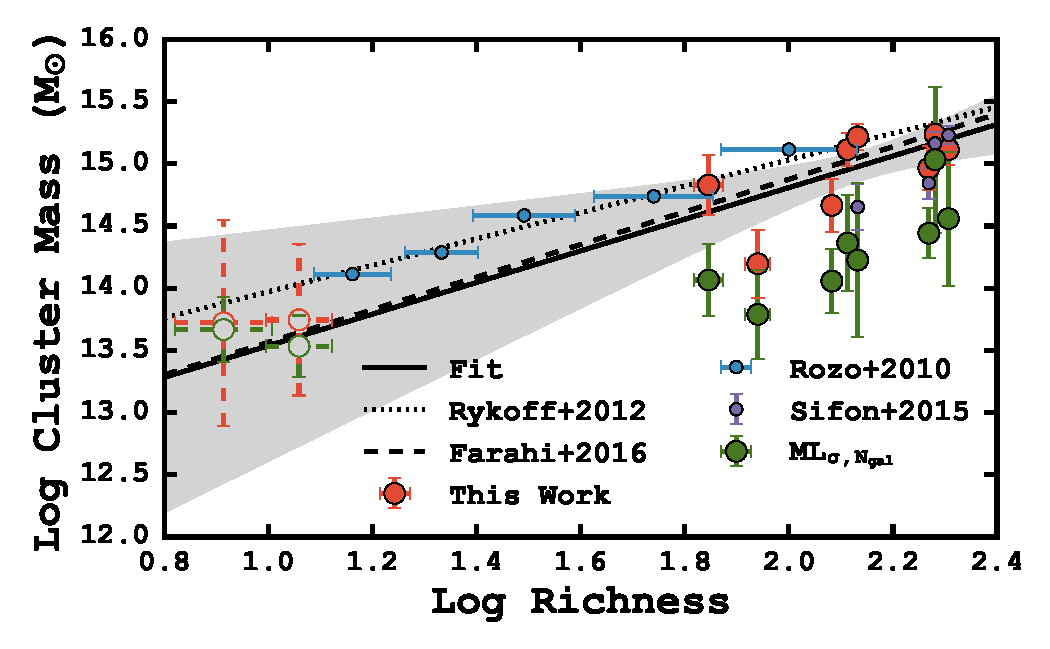
\includegraphics[width=\textwidth]{./figures2/massRichness.pdf} 
	\end{center}
	\caption{Richness, $\lambda$, versus total cluster mass for the clusters in our sample.} 
	The solid black like shows our best-fitting relation (Equation~\protect\ref{2eq: best fit}), the dashed line shows the relation from \protect\cite{Farahi2016}, and the dotted line shows the relation from \protect\cite{Rykoff2012}. The gray shaded region corresponds to the 68\% confidence area on our best-fit. We also include stacked WL masses from \protect\cite{Rozo2010} and the high-mass cluster mass estimates of \protect\cite{Sifon2015} for comparison.
\label{2fig:massRichness} 
\end{figure}

We found in \citetalias{Boada2016} that HETDEX will be able to accurately estimate the absolute calibration and intrinsic scatter of the optical-richness-cluster-mass relationship for a small range of intrinsic scatters. Here we use the ten clusters observed to do the same. For our cluster mass estimates we use the masses predicted by the power law relation given in Equation~\ref{2eq:power law}. 

To find a best-fitting richness-mass relation for our data we are required to fit $y=mx+b$ where $y$ is the predicted cluster mass and $x$ is the optical richness, considering measurement errors in richness and predicted cluster mass along with intrinsic scatter of the relation. We assume the intrinsic scatter is constant from point to point, and we assume (not necessarily correctly) that all measurement errors are Gaussian. With the assumption of all Gaussian scatters we have:
\begin{equation}\label{2eqn:intrinsic scatter}
	p(y_i|x_i) = \frac{1}{\sqrt{2\,\pi\,\sigma^2}}
	 \,\exp\left(-\frac{[y_i - m\,x_i - b]^2}{2\,\sigma^2}\right)
\end{equation}
for the intrinsic scatter,
\begin{equation}\label{2eqn:xerr}
	p(\hat{x_i}|x_i) = \frac{1}{\sqrt{2\,\pi\,\sigma_{x,i}^2}}
	 \,\exp\left(-\frac{[\hat{x_i} - x_i]^2}{2\,\sigma_{x,i}^2}\right)
\end{equation}
and
\begin{equation}\label{2eqn:yerr}
	p(\hat{y_i}|y_i) = \frac{1}{\sqrt{2\,\pi\,\sigma_{y,i}^2}}
	 \,\exp\left(-\frac{[\hat{y_i} -y_i]^2}{2\,\sigma_{y,i}^2}\right)
\end{equation}
for the measurement errors on the $x$ and $y$ variables respectively. We combine these three probabilities into
\begin{equation}
	p(\hat{y_i}|\hat{x_i}) = \int_{-\infty}^\infty dy_ip(\hat{y_i}|y_i) \int_{-\infty}^\infty dx_ip(y_i|x_i)p(x_i|\hat{x_i}).
\end{equation}
We assume flat priors on $x_i$ so that $p(x_i|\hat{x_i}) = p(\hat{x_i}|x_i)$ and substitute our probability equations from above. We find
\begin{equation}
	\begin{split}
	p(\hat{y_i}|\hat{x_i}) & = \\ 
	&\frac{1}{\sqrt{2\,\pi\,(\sigma^2 + \sigma_{y,i}^2 + m^2\sigma_{x,i}^2)}}\exp\left(-\frac{[y_i - m\,x_i - b]^2}{2\,(\sigma^2 + \sigma_{y,i}^2 + m^2\sigma_{x,i}^2)}\right)
	\end{split}
\end{equation}
which for $\sigma_{x,i}=0$ (no uncertainty on the independent variable) reduces to the familiar form of a Gaussian with a combination of measurement error and intrinsic scatter. We convert this probability function into a likelihood by taking the product of all the individual probabilities,  
\begin{equation}\label{2eq:like}
\mathscr{L} = \prod_{i=1}^N \ p(\hat{y_i}|\hat{x_i}).
\end{equation}
and maximize this likelihood by sampling from the posterior probability distribution. We quote the most probable slope and intercept as the median value of the posterior probability distributions with uncertainties as the square root of the second moment of the same distribution.

After fitting to the cluster masses in this work, we find a best fitting relation of
\begin{equation}\label{2eq: best fit}
 \mathrm{Log}\,M_{200c}=1.17\pm{0.39}\, \mathrm{Log}\,\lambda + 12.4863\pm{0.82}. 
\end{equation}
This best-fitting relation is shown in Figure~\ref{2fig:massRichness} where the large orange points are the power law estimated cluster masses from this work. The dotted and dashed lines show the richness-mass relations of \cite{Rykoff2012} and \cite{Farahi2016} respectively. The shaded region shows our $1\sigma$ confidence area of our best fit. We compare the properties of our optical richness-mass relation to others from the literature in the following subsection.

We can estimate the intrinsic scatter in the relation two ways. Because our generative model includes an intrinsic scatter term, we can use the MCMC samples directly. We find $\sigma_{M|\lambda} = 0.22\pm0.13$ dex. We can also calculate the standard deviation of the residuals, which gives  $\sigma_{M|\lambda} = 0.27\pm0.07$ dex. Both values fall into the range where HETDEX is most sensitive \citepalias{Boada2016}, which is encouraging for the larger survey. Both of these scatter estimates include all ten clusters. The two lowest mass clusters have significant uncertainties associated with their mass estimates. If we exclude the two low mass clusters, and c328p33+0p19 where we significantly underestimate the mass, the scatter for remaining seven clusters is $\sigma_{M|\lambda} = 0.24\pm0.09$ dex.

\subsection{Calibration of the Richness-Mass Relation}
Here we compare our fit of the richness-mass relation to a variety of constraints from the literature. Because we have selected our clusters from the redMapper catalog, we begin with the richness-mass relation from \cite{Rykoff2012}. The authors suggest a power law index of $\alpha=1.06$ and an absolute mass scale of Log $M_{200c}/\Msol=14.64$ at $\lambda=60$. We find a small difference in the slope, and a lower absolute mass scale of Log $M_{200c}/\Msol = 14.57\pm1.07$. Figure~\ref{2fig:massRichness} shows this difference. \cite{Rykoff2012} go on to note that their relationship should not be taken as a rigorously measured relationship, so this discrepancy is unsurprising. 

With very careful handling of uncertainties, \cite{Simet2016} find the a normalization of Log M/\Msol\ $=14.344\pm0.021$(statistical)$\pm0.023$(systematic) at $\lambda=40$ with a power-law index of $\alpha=1.33$\err{0.09}{0.10}. Our power law index is smaller, possibly due to the large errors (and few points in general) of the two low mass clusters. We find very good agreement with our reported value of Log $M_{200c}/\Msol = 14.36\pm1.03$

\cite{Farahi2016} has also calibrated the richness-mass relation of redMapper clusters through stacked LOSVD measurements. They report a power-law index of $\alpha=1.31\pm0.14$ and an absolute mass scale of Log $M_{200c}/\Msol = 14.19\pm0.10$, at $\lambda=30$, $z=0.2$ and assuming $h=0.7$. Again, while our slope is slightly misaligned with their reported value, we find excellent agreement in the absolute mass scale (see Figure~\ref{2fig:massRichness}).

While our reported absolute mass scale is very similar to those measured by recent studies, our measurement has quite a substantial uncertainty associated with it. This is due to the large uncertainty in the cluster mass estimate of the two XMM selected clusters. Coupled with so few clusters, in general, our fitting procedure cannot place tight constraints on the measured slope and intercept. With the many clusters expected to be observed with HETDEX these uncertainties should decrease significantly.  
Also promising is our measurement of the scatter about the best-fitting relation. \cite{Farahi2016, Simet2016} rely on stacked richness measurements to calibrate their relations. Here we use individual cluster mass measurements which enables us to better grasp the amount of intrinsic scatter. The scatter around the richness-mass relation for the redMapper clusters has been estimated to be $\sigma_{M|\lambda} \sim 0.2-0.3$ dex \citep{Rozo2014, Rozo2015}. This corresponds well to our estimate of $\sigma_{M|\lambda} \sim 0.25$ dex and the range most sensitively probed in our simulated HETDEX survey \citepalias{Boada2016}.

The ability of blind spectroscopy such as this to constrain all three parameters of interest to values similar to other studies is extremely positive for the potential of HETDEX. As cluster mass estimates become better constrained through the use of ML methods, we can expect to find even tighter constrains on the relation. This should lead to excellent calibration of other large-area sky surveys which produce optical photometry only. 

\section{Summary}\label{2sec:summary}
We carry out a proof-of-concept study where we present integral field unit observations with the Mitchelle Spectrograph of ten intermediate redshift ($z=0.2-0.3$) galaxy clusters. We observe cluster member galaxies within $R\sim0.5$ Mpc of each cluster, and determine each cluster's membership based on the line-of-sight velocity of each galaxy. The mass of each cluster is determined through a traditional power law and through a machine learning based approach. We use these estimates of cluster mass to measure the absolute mass scale and intrinsic scatter of the optical richness-cluster mass relationship. The goal of this study is to investigate how a blind spectroscopic survey, such as the forthcoming Hobby Eberly Dark Energy Experiment (HETDEX), will be able to predict cluster masses, and then to use those masses to help calibrate other observable-cluster mass scaling relations.
Our main results are as follows:
\begin{itemize}
	\item Using a power law scaling relation to estimate cluster mass from observed velocity dispersion, we find our galaxy clusters have masses $(0.52-17.37) \times 10^{14}$ \Msol\ ($M_{200c}$). The majority of these estimate are consistent with other published mass estimates which use a variety of estimation techniques. 
	\item The machine learning based approach of cluster mass estimation, while powerful, requires a deep understanding of both the machine learning algorithms available, and expert knowledge of the problem domain. We find that a suit of sample data drawn from a similarly sized cosmological volume is critical to the reliable prediction of cluster masses. When this is available, the predicted cluster masses show less bias and lower scatter compared to a traditional power law scaling relation.
	\item We fit a power law to all ten observed clusters which gives a best-fitting optical richness-mass relationship of:
		\begin{equation}
			\mathrm{Log}\,M_{200c}=1.17\pm{0.39}\, \mathrm{Log}\,\lambda + 12.4863\pm{0.82}. 
		\end{equation}
with an overall normalization of Log $M_{200c}/\Msol = 14.21\pm1.00$ at $\lambda=30$ and an intrinsic scatter $\sigma_{M|\lambda} \sim 0.25$. Both of these properties compare well to other recent richness-mass studies. This suggests that a survey such as HETDEX will be able to provide a crucial, independent, measurement of these uncertainties, to a much higher precision than is possible in this work. This bodes well for the success of HETDEX as not only a high redshift galaxy survey but as a important calibration tool for many large-area sky surveys for years to come.
\end{itemize}